\documentclass[twoside]{book}

% Packages required by doxygen
\usepackage{fixltx2e}
\usepackage{calc}
\usepackage{doxygen}
\usepackage[export]{adjustbox} % also loads graphicx
\usepackage{graphicx}
\usepackage[utf8]{inputenc}
\usepackage{makeidx}
\usepackage{multicol}
\usepackage{multirow}
\PassOptionsToPackage{warn}{textcomp}
\usepackage{textcomp}
\usepackage[nointegrals]{wasysym}
\usepackage[table]{xcolor}

% Font selection
\usepackage[T1]{fontenc}
\usepackage[scaled=.90]{helvet}
\usepackage{courier}
\usepackage{amssymb}
\usepackage{sectsty}
\renewcommand{\familydefault}{\sfdefault}
\allsectionsfont{%
  \fontseries{bc}\selectfont%
  \color{darkgray}%
}
\renewcommand{\DoxyLabelFont}{%
  \fontseries{bc}\selectfont%
  \color{darkgray}%
}
\newcommand{\+}{\discretionary{\mbox{\scriptsize$\hookleftarrow$}}{}{}}

% Page & text layout
\usepackage{geometry}
\geometry{%
  a4paper,%
  top=2.5cm,%
  bottom=2.5cm,%
  left=2.5cm,%
  right=2.5cm%
}
\tolerance=750
\hfuzz=15pt
\hbadness=750
\setlength{\emergencystretch}{15pt}
\setlength{\parindent}{0cm}
\setlength{\parskip}{3ex plus 2ex minus 2ex}
\makeatletter
\renewcommand{\paragraph}{%
  \@startsection{paragraph}{4}{0ex}{-1.0ex}{1.0ex}{%
    \normalfont\normalsize\bfseries\SS@parafont%
  }%
}
\renewcommand{\subparagraph}{%
  \@startsection{subparagraph}{5}{0ex}{-1.0ex}{1.0ex}{%
    \normalfont\normalsize\bfseries\SS@subparafont%
  }%
}
\makeatother

% Headers & footers
\usepackage{fancyhdr}
\pagestyle{fancyplain}
\fancyhead[LE]{\fancyplain{}{\bfseries\thepage}}
\fancyhead[CE]{\fancyplain{}{}}
\fancyhead[RE]{\fancyplain{}{\bfseries\leftmark}}
\fancyhead[LO]{\fancyplain{}{\bfseries\rightmark}}
\fancyhead[CO]{\fancyplain{}{}}
\fancyhead[RO]{\fancyplain{}{\bfseries\thepage}}
\fancyfoot[LE]{\fancyplain{}{}}
\fancyfoot[CE]{\fancyplain{}{}}
\fancyfoot[RE]{\fancyplain{}{\bfseries\scriptsize Generated by Doxygen }}
\fancyfoot[LO]{\fancyplain{}{\bfseries\scriptsize Generated by Doxygen }}
\fancyfoot[CO]{\fancyplain{}{}}
\fancyfoot[RO]{\fancyplain{}{}}
\renewcommand{\footrulewidth}{0.4pt}
\renewcommand{\chaptermark}[1]{%
  \markboth{#1}{}%
}
\renewcommand{\sectionmark}[1]{%
  \markright{\thesection\ #1}%
}

% Indices & bibliography
\usepackage{natbib}
\usepackage[titles]{tocloft}
\setcounter{tocdepth}{3}
\setcounter{secnumdepth}{5}
\makeindex

% Hyperlinks (required, but should be loaded last)
\usepackage{ifpdf}
\ifpdf
  \usepackage[pdftex,pagebackref=true]{hyperref}
\else
  \usepackage[ps2pdf,pagebackref=true]{hyperref}
\fi
\hypersetup{%
  colorlinks=true,%
  linkcolor=blue,%
  citecolor=blue,%
  unicode%
}

% Custom commands
\newcommand{\clearemptydoublepage}{%
  \newpage{\pagestyle{empty}\cleardoublepage}%
}

\usepackage{caption}
\captionsetup{labelsep=space,justification=centering,font={bf},singlelinecheck=off,skip=4pt,position=top}

%===== C O N T E N T S =====

\begin{document}

% Titlepage & ToC
\hypersetup{pageanchor=false,
             bookmarksnumbered=true,
             pdfencoding=unicode
            }
\pagenumbering{alph}
\begin{titlepage}
\vspace*{7cm}
\begin{center}%
{\Large Spherical histogramm }\\
\vspace*{1cm}
{\large Generated by Doxygen 1.8.13}\\
\end{center}
\end{titlepage}
\clearemptydoublepage
\pagenumbering{roman}
\tableofcontents
\clearemptydoublepage
\pagenumbering{arabic}
\hypersetup{pageanchor=true}

%--- Begin generated contents ---
\chapter{Namespace Index}
\input{namespaces}
\chapter{Hierarchical Index}
\section{Class Hierarchy}
This inheritance list is sorted roughly, but not completely, alphabetically\+:\begin{DoxyCompactList}
\item Q\+Main\+Window\begin{DoxyCompactList}
\item \contentsline{section}{Main\+Window}{\pageref{class_main_window}}{}
\end{DoxyCompactList}
\item Q\+Open\+G\+L\+Functions\begin{DoxyCompactList}
\item \contentsline{section}{Sphere\+Widget}{\pageref{class_sphere_widget}}{}
\end{DoxyCompactList}
\item Q\+Open\+G\+L\+Widget\begin{DoxyCompactList}
\item \contentsline{section}{Sphere\+Widget}{\pageref{class_sphere_widget}}{}
\end{DoxyCompactList}
\item \contentsline{section}{Render\+Data}{\pageref{class_render_data}}{}
\item \contentsline{section}{Sphere\+Depth\+Data}{\pageref{struct_sphere_depth_data}}{}
\end{DoxyCompactList}

\chapter{Class Index}
\section{Class List}
Here are the classes, structs, unions and interfaces with brief descriptions\+:\begin{DoxyCompactList}
\item\contentsline{section}{\hyperlink{class_main_window}{Main\+Window} }{\pageref{class_main_window}}{}
\item\contentsline{section}{\hyperlink{class_render_data}{Render\+Data} \\*Singleton that stores and calculates all logical application data }{\pageref{class_render_data}}{}
\item\contentsline{section}{\hyperlink{struct_sphere_depth_data}{Sphere\+Depth\+Data} }{\pageref{struct_sphere_depth_data}}{}
\item\contentsline{section}{\hyperlink{class_sphere_widget}{Sphere\+Widget} }{\pageref{class_sphere_widget}}{}
\end{DoxyCompactList}

\chapter{File Index}
\section{File List}
Here is a list of all files with brief descriptions\+:\begin{DoxyCompactList}
\item\contentsline{section}{\hyperlink{main_8cpp}{main.\+cpp} }{\pageref{main_8cpp}}{}
\item\contentsline{section}{\hyperlink{mainwindow_8cpp}{mainwindow.\+cpp} }{\pageref{mainwindow_8cpp}}{}
\item\contentsline{section}{\hyperlink{mainwindow_8h}{mainwindow.\+h} }{\pageref{mainwindow_8h}}{}
\item\contentsline{section}{\hyperlink{renderdata_8cpp}{renderdata.\+cpp} }{\pageref{renderdata_8cpp}}{}
\item\contentsline{section}{\hyperlink{renderdata_8h}{renderdata.\+h} }{\pageref{renderdata_8h}}{}
\item\contentsline{section}{\hyperlink{spheredepthdata_8cpp}{spheredepthdata.\+cpp} }{\pageref{spheredepthdata_8cpp}}{}
\item\contentsline{section}{\hyperlink{spheredepthdata_8h}{spheredepthdata.\+h} }{\pageref{spheredepthdata_8h}}{}
\item\contentsline{section}{\hyperlink{spherewidget_8cpp}{spherewidget.\+cpp} }{\pageref{spherewidget_8cpp}}{}
\item\contentsline{section}{\hyperlink{spherewidget_8h}{spherewidget.\+h} }{\pageref{spherewidget_8h}}{}
\item\contentsline{section}{resources/\hyperlink{colormaps__matplotlib_8h}{colormaps\+\_\+matplotlib.\+h} }{\pageref{colormaps__matplotlib_8h}}{}
\end{DoxyCompactList}

\chapter{Namespace Documentation}
\hypertarget{namespacecm}{}\section{cm Namespace Reference}
\label{namespacecm}\index{cm@{cm}}
\subsection*{Enumerations}
\begin{DoxyCompactItemize}
\item 
enum \hyperlink{namespacecm_aabaf84796e8a93bd6adca4c5bdea5311}{Color\+Map\+Name} \{ \newline
\hyperlink{namespacecm_aabaf84796e8a93bd6adca4c5bdea5311a64c2ad47aeb457c258518a5318ed071d}{Color\+Map\+Name\+::\+Cividis} = 0, 
\hyperlink{namespacecm_aabaf84796e8a93bd6adca4c5bdea5311a8bb279f735c1d9c831e935cca2613b58}{Color\+Map\+Name\+::\+Inferno} = 1, 
\hyperlink{namespacecm_aabaf84796e8a93bd6adca4c5bdea5311a1b62e99f86d45e754e5e79d9fa9dfcde}{Color\+Map\+Name\+::\+Magma} = 2, 
\hyperlink{namespacecm_aabaf84796e8a93bd6adca4c5bdea5311ab20a4217acaf4316739c6a5f6679ef60}{Color\+Map\+Name\+::\+Plasma} = 3, 
\newline
\hyperlink{namespacecm_aabaf84796e8a93bd6adca4c5bdea5311a6f53bfe04e78da893ba0c4f35ba6847e}{Color\+Map\+Name\+::\+Turbo} = 4, 
\hyperlink{namespacecm_aabaf84796e8a93bd6adca4c5bdea5311a951ee92ee5e947e1e7e1cb6376523c1a}{Color\+Map\+Name\+::\+Viridis} = 5
 \}
\end{DoxyCompactItemize}
\subsection*{Variables}
\begin{DoxyCompactItemize}
\item 
const std\+::unordered\+\_\+map$<$ std\+::string, \hyperlink{namespacecm_aabaf84796e8a93bd6adca4c5bdea5311}{Color\+Map\+Name} $>$ \hyperlink{namespacecm_a62bba085a1fd823321f70d53df62ed53}{string\+To\+Color\+Enum}
\item 
const float \hyperlink{namespacecm_a6c7ebc740c952f5ae2569bbc4d6b0ba3}{\+\_\+magma\+\_\+data} \mbox{[}3 $\ast$256\mbox{]}
\item 
const float \hyperlink{namespacecm_abd85098a9455ec3b6a1367e717904d81}{\+\_\+inferno\+\_\+data} \mbox{[}3 $\ast$256\mbox{]}
\item 
const float \hyperlink{namespacecm_a5e6bdf45c99146f14941db900036b42c}{\+\_\+plasma\+\_\+data} \mbox{[}3 $\ast$256\mbox{]}
\item 
const float \hyperlink{namespacecm_af931122787ac6cf5d5c8d834adcb3fc8}{\+\_\+viridis\+\_\+data} \mbox{[}3 $\ast$256\mbox{]}
\item 
const float \hyperlink{namespacecm_a9aebd281c6d694ef79eb8f989866ff6d}{\+\_\+cividis\+\_\+data} \mbox{[}3 $\ast$256\mbox{]}
\item 
const float \hyperlink{namespacecm_a1394411b557deb7b6f8c58a9c39ff4a3}{\+\_\+turbo\+\_\+data} \mbox{[}3 $\ast$256\mbox{]}
\end{DoxyCompactItemize}


\subsection{Enumeration Type Documentation}
\mbox{\Hypertarget{namespacecm_aabaf84796e8a93bd6adca4c5bdea5311}\label{namespacecm_aabaf84796e8a93bd6adca4c5bdea5311}} 
\index{cm@{cm}!Color\+Map\+Name@{Color\+Map\+Name}}
\index{Color\+Map\+Name@{Color\+Map\+Name}!cm@{cm}}
\subsubsection{\texorpdfstring{Color\+Map\+Name}{ColorMapName}}
{\footnotesize\ttfamily enum \hyperlink{namespacecm_aabaf84796e8a93bd6adca4c5bdea5311}{cm\+::\+Color\+Map\+Name}\hspace{0.3cm}{\ttfamily [strong]}}

Describes all available color maps \begin{DoxyEnumFields}{Enumerator}
\raisebox{\heightof{T}}[0pt][0pt]{\index{Cividis@{Cividis}!cm@{cm}}\index{cm@{cm}!Cividis@{Cividis}}}\mbox{\Hypertarget{namespacecm_aabaf84796e8a93bd6adca4c5bdea5311a64c2ad47aeb457c258518a5318ed071d}\label{namespacecm_aabaf84796e8a93bd6adca4c5bdea5311a64c2ad47aeb457c258518a5318ed071d}} 
Cividis&\\
\hline

\raisebox{\heightof{T}}[0pt][0pt]{\index{Inferno@{Inferno}!cm@{cm}}\index{cm@{cm}!Inferno@{Inferno}}}\mbox{\Hypertarget{namespacecm_aabaf84796e8a93bd6adca4c5bdea5311a8bb279f735c1d9c831e935cca2613b58}\label{namespacecm_aabaf84796e8a93bd6adca4c5bdea5311a8bb279f735c1d9c831e935cca2613b58}} 
Inferno&\\
\hline

\raisebox{\heightof{T}}[0pt][0pt]{\index{Magma@{Magma}!cm@{cm}}\index{cm@{cm}!Magma@{Magma}}}\mbox{\Hypertarget{namespacecm_aabaf84796e8a93bd6adca4c5bdea5311a1b62e99f86d45e754e5e79d9fa9dfcde}\label{namespacecm_aabaf84796e8a93bd6adca4c5bdea5311a1b62e99f86d45e754e5e79d9fa9dfcde}} 
Magma&\\
\hline

\raisebox{\heightof{T}}[0pt][0pt]{\index{Plasma@{Plasma}!cm@{cm}}\index{cm@{cm}!Plasma@{Plasma}}}\mbox{\Hypertarget{namespacecm_aabaf84796e8a93bd6adca4c5bdea5311ab20a4217acaf4316739c6a5f6679ef60}\label{namespacecm_aabaf84796e8a93bd6adca4c5bdea5311ab20a4217acaf4316739c6a5f6679ef60}} 
Plasma&\\
\hline

\raisebox{\heightof{T}}[0pt][0pt]{\index{Turbo@{Turbo}!cm@{cm}}\index{cm@{cm}!Turbo@{Turbo}}}\mbox{\Hypertarget{namespacecm_aabaf84796e8a93bd6adca4c5bdea5311a6f53bfe04e78da893ba0c4f35ba6847e}\label{namespacecm_aabaf84796e8a93bd6adca4c5bdea5311a6f53bfe04e78da893ba0c4f35ba6847e}} 
Turbo&\\
\hline

\raisebox{\heightof{T}}[0pt][0pt]{\index{Viridis@{Viridis}!cm@{cm}}\index{cm@{cm}!Viridis@{Viridis}}}\mbox{\Hypertarget{namespacecm_aabaf84796e8a93bd6adca4c5bdea5311a951ee92ee5e947e1e7e1cb6376523c1a}\label{namespacecm_aabaf84796e8a93bd6adca4c5bdea5311a951ee92ee5e947e1e7e1cb6376523c1a}} 
Viridis&\\
\hline

\end{DoxyEnumFields}


Definition at line 13 of file colormaps\+\_\+matplotlib.\+h.



\subsection{Variable Documentation}
\mbox{\Hypertarget{namespacecm_a9aebd281c6d694ef79eb8f989866ff6d}\label{namespacecm_a9aebd281c6d694ef79eb8f989866ff6d}} 
\index{cm@{cm}!\+\_\+cividis\+\_\+data@{\+\_\+cividis\+\_\+data}}
\index{\+\_\+cividis\+\_\+data@{\+\_\+cividis\+\_\+data}!cm@{cm}}
\subsubsection{\texorpdfstring{\+\_\+cividis\+\_\+data}{\_cividis\_data}}
{\footnotesize\ttfamily const float cm\+::\+\_\+cividis\+\_\+data\mbox{[}3 $\ast$256\mbox{]}}



Definition at line 1056 of file colormaps\+\_\+matplotlib.\+h.

\mbox{\Hypertarget{namespacecm_abd85098a9455ec3b6a1367e717904d81}\label{namespacecm_abd85098a9455ec3b6a1367e717904d81}} 
\index{cm@{cm}!\+\_\+inferno\+\_\+data@{\+\_\+inferno\+\_\+data}}
\index{\+\_\+inferno\+\_\+data@{\+\_\+inferno\+\_\+data}!cm@{cm}}
\subsubsection{\texorpdfstring{\+\_\+inferno\+\_\+data}{\_inferno\_data}}
{\footnotesize\ttfamily const float cm\+::\+\_\+inferno\+\_\+data\mbox{[}3 $\ast$256\mbox{]}}



Definition at line 285 of file colormaps\+\_\+matplotlib.\+h.

\mbox{\Hypertarget{namespacecm_a6c7ebc740c952f5ae2569bbc4d6b0ba3}\label{namespacecm_a6c7ebc740c952f5ae2569bbc4d6b0ba3}} 
\index{cm@{cm}!\+\_\+magma\+\_\+data@{\+\_\+magma\+\_\+data}}
\index{\+\_\+magma\+\_\+data@{\+\_\+magma\+\_\+data}!cm@{cm}}
\subsubsection{\texorpdfstring{\+\_\+magma\+\_\+data}{\_magma\_data}}
{\footnotesize\ttfamily const float cm\+::\+\_\+magma\+\_\+data\mbox{[}3 $\ast$256\mbox{]}}



Definition at line 28 of file colormaps\+\_\+matplotlib.\+h.

\mbox{\Hypertarget{namespacecm_a5e6bdf45c99146f14941db900036b42c}\label{namespacecm_a5e6bdf45c99146f14941db900036b42c}} 
\index{cm@{cm}!\+\_\+plasma\+\_\+data@{\+\_\+plasma\+\_\+data}}
\index{\+\_\+plasma\+\_\+data@{\+\_\+plasma\+\_\+data}!cm@{cm}}
\subsubsection{\texorpdfstring{\+\_\+plasma\+\_\+data}{\_plasma\_data}}
{\footnotesize\ttfamily const float cm\+::\+\_\+plasma\+\_\+data\mbox{[}3 $\ast$256\mbox{]}}



Definition at line 542 of file colormaps\+\_\+matplotlib.\+h.

\mbox{\Hypertarget{namespacecm_a1394411b557deb7b6f8c58a9c39ff4a3}\label{namespacecm_a1394411b557deb7b6f8c58a9c39ff4a3}} 
\index{cm@{cm}!\+\_\+turbo\+\_\+data@{\+\_\+turbo\+\_\+data}}
\index{\+\_\+turbo\+\_\+data@{\+\_\+turbo\+\_\+data}!cm@{cm}}
\subsubsection{\texorpdfstring{\+\_\+turbo\+\_\+data}{\_turbo\_data}}
{\footnotesize\ttfamily const float cm\+::\+\_\+turbo\+\_\+data\mbox{[}3 $\ast$256\mbox{]}}



Definition at line 1313 of file colormaps\+\_\+matplotlib.\+h.

\mbox{\Hypertarget{namespacecm_af931122787ac6cf5d5c8d834adcb3fc8}\label{namespacecm_af931122787ac6cf5d5c8d834adcb3fc8}} 
\index{cm@{cm}!\+\_\+viridis\+\_\+data@{\+\_\+viridis\+\_\+data}}
\index{\+\_\+viridis\+\_\+data@{\+\_\+viridis\+\_\+data}!cm@{cm}}
\subsubsection{\texorpdfstring{\+\_\+viridis\+\_\+data}{\_viridis\_data}}
{\footnotesize\ttfamily const float cm\+::\+\_\+viridis\+\_\+data\mbox{[}3 $\ast$256\mbox{]}}



Definition at line 799 of file colormaps\+\_\+matplotlib.\+h.

\mbox{\Hypertarget{namespacecm_a62bba085a1fd823321f70d53df62ed53}\label{namespacecm_a62bba085a1fd823321f70d53df62ed53}} 
\index{cm@{cm}!string\+To\+Color\+Enum@{string\+To\+Color\+Enum}}
\index{string\+To\+Color\+Enum@{string\+To\+Color\+Enum}!cm@{cm}}
\subsubsection{\texorpdfstring{string\+To\+Color\+Enum}{stringToColorEnum}}
{\footnotesize\ttfamily const std\+::unordered\+\_\+map$<$std\+::string, \hyperlink{namespacecm_aabaf84796e8a93bd6adca4c5bdea5311}{Color\+Map\+Name}$>$ cm\+::string\+To\+Color\+Enum}

{\bfseries Initial value\+:}
\begin{DoxyCode}
= \{
    \{\textcolor{stringliteral}{"Cividis"}, \hyperlink{namespacecm_aabaf84796e8a93bd6adca4c5bdea5311a64c2ad47aeb457c258518a5318ed071d}{cm::ColorMapName::Cividis}\},
    \{\textcolor{stringliteral}{"Inferno"}, \hyperlink{namespacecm_aabaf84796e8a93bd6adca4c5bdea5311a8bb279f735c1d9c831e935cca2613b58}{cm::ColorMapName::Inferno}\},
    \{\textcolor{stringliteral}{"Magma"}, \hyperlink{namespacecm_aabaf84796e8a93bd6adca4c5bdea5311a1b62e99f86d45e754e5e79d9fa9dfcde}{cm::ColorMapName::Magma}\},
    \{\textcolor{stringliteral}{"Plasma"}, \hyperlink{namespacecm_aabaf84796e8a93bd6adca4c5bdea5311ab20a4217acaf4316739c6a5f6679ef60}{cm::ColorMapName::Plasma}\},
    \{\textcolor{stringliteral}{"Turbo"}, \hyperlink{namespacecm_aabaf84796e8a93bd6adca4c5bdea5311a6f53bfe04e78da893ba0c4f35ba6847e}{cm::ColorMapName::Turbo}\},
    \{\textcolor{stringliteral}{"Viridis"}, \hyperlink{namespacecm_aabaf84796e8a93bd6adca4c5bdea5311a951ee92ee5e947e1e7e1cb6376523c1a}{cm::ColorMapName::Viridis}\},
\}
\end{DoxyCode}
For conveniently retrieving colormap enum values from their string representation 

Definition at line 16 of file colormaps\+\_\+matplotlib.\+h.


\input{dc/df0/namespace_ui}
\chapter{Class Documentation}
\hypertarget{class_main_window}{}\section{Main\+Window Class Reference}
\label{class_main_window}\index{Main\+Window@{Main\+Window}}


{\ttfamily \#include $<$mainwindow.\+h$>$}



Inheritance diagram for Main\+Window\+:\nopagebreak
\begin{figure}[H]
\begin{center}
\leavevmode
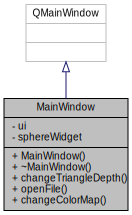
\includegraphics[width=204pt]{class_main_window__inherit__graph}
\end{center}
\end{figure}


Collaboration diagram for Main\+Window\+:
\nopagebreak
\begin{figure}[H]
\begin{center}
\leavevmode
\includegraphics[width=350pt]{class_main_window__coll__graph}
\end{center}
\end{figure}
\subsection*{Public Slots}
\begin{DoxyCompactItemize}
\item 
void \hyperlink{class_main_window_a7bdf36376a7474c5218923ed66baa937}{change\+Triangle\+Depth} (int depth)
\item 
void \hyperlink{class_main_window_a288b768c3c21a9171bdc56fe845ece8b}{open\+File} ()
\item 
void \hyperlink{class_main_window_a1cfcf14a3dbba8db45a2444a0fbe5a9f}{change\+Color\+Map} (Q\+String map\+Name)
\end{DoxyCompactItemize}
\subsection*{Public Member Functions}
\begin{DoxyCompactItemize}
\item 
\hyperlink{class_main_window_a8b244be8b7b7db1b08de2a2acb9409db}{Main\+Window} (Q\+Widget $\ast$parent=0)
\item 
\hyperlink{class_main_window_ae98d00a93bc118200eeef9f9bba1dba7}{$\sim$\+Main\+Window} ()
\end{DoxyCompactItemize}
\subsection*{Private Attributes}
\begin{DoxyCompactItemize}
\item 
Ui\+::\+Main\+Window $\ast$ \hyperlink{class_main_window_a35466a70ed47252a0191168126a352a5}{ui}
\item 
\hyperlink{class_sphere_widget}{Sphere\+Widget} $\ast$ \hyperlink{class_main_window_afc60f18ae3cf60a9c231d8344a5bbda8}{sphere\+Widget}
\end{DoxyCompactItemize}


\subsection{Detailed Description}


Definition at line 14 of file mainwindow.\+h.



\subsection{Constructor \& Destructor Documentation}
\mbox{\Hypertarget{class_main_window_a8b244be8b7b7db1b08de2a2acb9409db}\label{class_main_window_a8b244be8b7b7db1b08de2a2acb9409db}} 
\index{Main\+Window@{Main\+Window}!Main\+Window@{Main\+Window}}
\index{Main\+Window@{Main\+Window}!Main\+Window@{Main\+Window}}
\subsubsection{\texorpdfstring{Main\+Window()}{MainWindow()}}
{\footnotesize\ttfamily Main\+Window\+::\+Main\+Window (\begin{DoxyParamCaption}\item[{Q\+Widget $\ast$}]{parent = {\ttfamily 0} }\end{DoxyParamCaption})\hspace{0.3cm}{\ttfamily [explicit]}}



Definition at line 6 of file mainwindow.\+cpp.

\mbox{\Hypertarget{class_main_window_ae98d00a93bc118200eeef9f9bba1dba7}\label{class_main_window_ae98d00a93bc118200eeef9f9bba1dba7}} 
\index{Main\+Window@{Main\+Window}!````~Main\+Window@{$\sim$\+Main\+Window}}
\index{````~Main\+Window@{$\sim$\+Main\+Window}!Main\+Window@{Main\+Window}}
\subsubsection{\texorpdfstring{$\sim$\+Main\+Window()}{~MainWindow()}}
{\footnotesize\ttfamily Main\+Window\+::$\sim$\+Main\+Window (\begin{DoxyParamCaption}{ }\end{DoxyParamCaption})}



Definition at line 22 of file mainwindow.\+cpp.



\subsection{Member Function Documentation}
\mbox{\Hypertarget{class_main_window_a1cfcf14a3dbba8db45a2444a0fbe5a9f}\label{class_main_window_a1cfcf14a3dbba8db45a2444a0fbe5a9f}} 
\index{Main\+Window@{Main\+Window}!change\+Color\+Map@{change\+Color\+Map}}
\index{change\+Color\+Map@{change\+Color\+Map}!Main\+Window@{Main\+Window}}
\subsubsection{\texorpdfstring{change\+Color\+Map}{changeColorMap}}
{\footnotesize\ttfamily void Main\+Window\+::change\+Color\+Map (\begin{DoxyParamCaption}\item[{Q\+String}]{map\+Name }\end{DoxyParamCaption})\hspace{0.3cm}{\ttfamily [slot]}}



Definition at line 46 of file mainwindow.\+cpp.

\mbox{\Hypertarget{class_main_window_a7bdf36376a7474c5218923ed66baa937}\label{class_main_window_a7bdf36376a7474c5218923ed66baa937}} 
\index{Main\+Window@{Main\+Window}!change\+Triangle\+Depth@{change\+Triangle\+Depth}}
\index{change\+Triangle\+Depth@{change\+Triangle\+Depth}!Main\+Window@{Main\+Window}}
\subsubsection{\texorpdfstring{change\+Triangle\+Depth}{changeTriangleDepth}}
{\footnotesize\ttfamily void Main\+Window\+::change\+Triangle\+Depth (\begin{DoxyParamCaption}\item[{int}]{depth }\end{DoxyParamCaption})\hspace{0.3cm}{\ttfamily [slot]}}



Definition at line 28 of file mainwindow.\+cpp.

\mbox{\Hypertarget{class_main_window_a288b768c3c21a9171bdc56fe845ece8b}\label{class_main_window_a288b768c3c21a9171bdc56fe845ece8b}} 
\index{Main\+Window@{Main\+Window}!open\+File@{open\+File}}
\index{open\+File@{open\+File}!Main\+Window@{Main\+Window}}
\subsubsection{\texorpdfstring{open\+File}{openFile}}
{\footnotesize\ttfamily void Main\+Window\+::open\+File (\begin{DoxyParamCaption}{ }\end{DoxyParamCaption})\hspace{0.3cm}{\ttfamily [slot]}}



Definition at line 34 of file mainwindow.\+cpp.



\subsection{Member Data Documentation}
\mbox{\Hypertarget{class_main_window_afc60f18ae3cf60a9c231d8344a5bbda8}\label{class_main_window_afc60f18ae3cf60a9c231d8344a5bbda8}} 
\index{Main\+Window@{Main\+Window}!sphere\+Widget@{sphere\+Widget}}
\index{sphere\+Widget@{sphere\+Widget}!Main\+Window@{Main\+Window}}
\subsubsection{\texorpdfstring{sphere\+Widget}{sphereWidget}}
{\footnotesize\ttfamily \hyperlink{class_sphere_widget}{Sphere\+Widget}$\ast$ Main\+Window\+::sphere\+Widget\hspace{0.3cm}{\ttfamily [private]}}



Definition at line 29 of file mainwindow.\+h.

\mbox{\Hypertarget{class_main_window_a35466a70ed47252a0191168126a352a5}\label{class_main_window_a35466a70ed47252a0191168126a352a5}} 
\index{Main\+Window@{Main\+Window}!ui@{ui}}
\index{ui@{ui}!Main\+Window@{Main\+Window}}
\subsubsection{\texorpdfstring{ui}{ui}}
{\footnotesize\ttfamily Ui\+::\+Main\+Window$\ast$ Main\+Window\+::ui\hspace{0.3cm}{\ttfamily [private]}}



Definition at line 28 of file mainwindow.\+h.



The documentation for this class was generated from the following files\+:\begin{DoxyCompactItemize}
\item 
\hyperlink{mainwindow_8h}{mainwindow.\+h}\item 
\hyperlink{mainwindow_8cpp}{mainwindow.\+cpp}\end{DoxyCompactItemize}

\hypertarget{class_render_data}{}\section{Render\+Data Class Reference}
\label{class_render_data}\index{Render\+Data@{Render\+Data}}


{\ttfamily \#include $<$renderdata.\+h$>$}

\subsection*{Public Member Functions}
\begin{DoxyCompactItemize}
\item 
\mbox{\Hypertarget{class_render_data_aa07295cc6e370997b02e68c917ff05de}\label{class_render_data_aa07295cc6e370997b02e68c917ff05de}} 
short {\bfseries get\+Current\+Sphere\+Depth} () const
\item 
\mbox{\Hypertarget{class_render_data_aabd6bd86800c7fc53788ef92ccf1ceb8}\label{class_render_data_aabd6bd86800c7fc53788ef92ccf1ceb8}} 
const float $\ast$ {\bfseries get\+Color\+Map} () const
\item 
\mbox{\Hypertarget{class_render_data_a9683c1cf21e861efaf1f7c1b7aaa2cf9}\label{class_render_data_a9683c1cf21e861efaf1f7c1b7aaa2cf9}} 
std\+::vector$<$ float $>$ {\bfseries get\+Points\+As\+Vector} (void)
\item 
\mbox{\Hypertarget{class_render_data_ac3ddb0af8cf9a0f2fb4d69815cf76b9d}\label{class_render_data_ac3ddb0af8cf9a0f2fb4d69815cf76b9d}} 
std\+::list$<$ Q\+Vector3D $>$ {\bfseries get\+Points} ()
\item 
\mbox{\Hypertarget{class_render_data_a9896a3ed194123ccf5cca42012d4b5e5}\label{class_render_data_a9896a3ed194123ccf5cca42012d4b5e5}} 
const std\+::vector$<$ float $>$ {\bfseries get\+Triangle\+Vertices\+And\+Colors\+At\+Current\+Depth} ()
\item 
\mbox{\Hypertarget{class_render_data_a58fe3351334cd518b930dfe0a0aa8732}\label{class_render_data_a58fe3351334cd518b930dfe0a0aa8732}} 
std\+::vector$<$ float $>$ {\bfseries get\+Colors\+For\+Triangles} (float alpha=1)
\item 
\mbox{\Hypertarget{class_render_data_a8cd691fd6f3cfbd22a1b84daffd2dba2}\label{class_render_data_a8cd691fd6f3cfbd22a1b84daffd2dba2}} 
std\+::vector$<$ float $>$ {\bfseries get\+Vertices\+At\+Current\+Depth} ()
\item 
\mbox{\Hypertarget{class_render_data_a8d5f7285d29dc9ca0f93fcf2b5826283}\label{class_render_data_a8d5f7285d29dc9ca0f93fcf2b5826283}} 
void {\bfseries set\+Sphere\+Depth} (short depth)
\item 
\mbox{\Hypertarget{class_render_data_adb1961bf93370d67c9efb416fde8fefb}\label{class_render_data_adb1961bf93370d67c9efb416fde8fefb}} 
void {\bfseries set\+Color\+Map} (Q\+String color\+Map\+Name)
\item 
void \hyperlink{class_render_data_ac161f29f7d6ae6fd3912e8af7bdccdfd}{load\+Points\+From\+File} (std\+::string filename)
\end{DoxyCompactItemize}
\subsection*{Static Public Member Functions}
\begin{DoxyCompactItemize}
\item 
\mbox{\Hypertarget{class_render_data_a1fffc72f3dd17ab052d4fb2f025ef5a0}\label{class_render_data_a1fffc72f3dd17ab052d4fb2f025ef5a0}} 
static \hyperlink{class_render_data}{Render\+Data} $\ast$ {\bfseries get\+Instance} ()
\end{DoxyCompactItemize}
\subsection*{Friends}
\begin{DoxyCompactItemize}
\item 
\mbox{\Hypertarget{class_render_data_aae9e6e2f2e7f9a8cde35b65facc0750b}\label{class_render_data_aae9e6e2f2e7f9a8cde35b65facc0750b}} 
class {\bfseries Icosphere}
\end{DoxyCompactItemize}


\subsection{Detailed Description}
Singleton to calculate and store data of the
\begin{DoxyItemize}
\item points currently loaded
\item icosphere in various depths
\item current rendering depth
\item currently used colormap
\item color of the icosphere triangles according to the respective point count 
\end{DoxyItemize}

\subsection{Member Function Documentation}
\mbox{\Hypertarget{class_render_data_ac161f29f7d6ae6fd3912e8af7bdccdfd}\label{class_render_data_ac161f29f7d6ae6fd3912e8af7bdccdfd}} 
\index{Render\+Data@{Render\+Data}!load\+Points\+From\+File@{load\+Points\+From\+File}}
\index{load\+Points\+From\+File@{load\+Points\+From\+File}!Render\+Data@{Render\+Data}}
\subsubsection{\texorpdfstring{load\+Points\+From\+File()}{loadPointsFromFile()}}
{\footnotesize\ttfamily void Render\+Data\+::load\+Points\+From\+File (\begin{DoxyParamCaption}\item[{std\+::string}]{filename }\end{DoxyParamCaption})}

Loads data points from given .npy-\/file containing a double precision Nx3-\/\+Numpy-\/array, passes them to Spherewidget in a render-\/friendly form and notifies the Icosphere to re-\/calculate the respective colors 

The documentation for this class was generated from the following files\+:\begin{DoxyCompactItemize}
\item 
renderdata.\+h\item 
renderdata.\+cpp\end{DoxyCompactItemize}

\hypertarget{struct_sphere_depth_data}{}\section{Sphere\+Depth\+Data Struct Reference}
\label{struct_sphere_depth_data}\index{Sphere\+Depth\+Data@{Sphere\+Depth\+Data}}


{\ttfamily \#include $<$spheredepthdata.\+h$>$}



Collaboration diagram for Sphere\+Depth\+Data\+:\nopagebreak
\begin{figure}[H]
\begin{center}
\leavevmode
\includegraphics[width=234pt]{d1/d26/struct_sphere_depth_data__coll__graph}
\end{center}
\end{figure}
\subsection*{Public Member Functions}
\begin{DoxyCompactItemize}
\item 
\hyperlink{struct_sphere_depth_data_adf3b418ea38626e3d768240d257504ea}{Sphere\+Depth\+Data} ()=default
\item 
\hyperlink{struct_sphere_depth_data_a746de4be5c4ff2bdcbdc1517aa88a4d9}{Sphere\+Depth\+Data} (short \hyperlink{struct_sphere_depth_data_a32dc63866d12b3102942e14bb28238ff}{depth}, std\+::vector$<$ float $>$ \hyperlink{struct_sphere_depth_data_a139a9131aa15308e012fc8190de2011d}{vertices}, std\+::vector$<$ std\+::list$<$ Q\+Vector3D $>$ $>$ \hyperlink{struct_sphere_depth_data_a9decfacc00300c153ecff80288b7413f}{points\+Per\+Triangle})
\item 
short \hyperlink{struct_sphere_depth_data_a925a7e0a5486b49151d823471ebe7fe6}{get\+Depth} () const
\item 
size\+\_\+t \hyperlink{struct_sphere_depth_data_ad151dd50ed037d91aecec6b285a3e342}{get\+Max\+Points\+Per\+Triangle} ()
\item 
std\+::vector$<$ std\+::list$<$ Q\+Vector3D $>$ $>$ \hyperlink{struct_sphere_depth_data_af42bd1ede7948a735367755a61148adc}{get\+Points\+Per\+Triangle} () const
\item 
std\+::vector$<$ float $>$ \hyperlink{struct_sphere_depth_data_adab658de163c515ec9a41a70300a0af9}{get\+Vertices} () const
\item 
bool \hyperlink{struct_sphere_depth_data_acdda270334d050e23b82ad0f700c5c1c}{is\+Empty} () const
\item 
void \hyperlink{struct_sphere_depth_data_a95e070bea3d8ec4a0449044e4616208f}{set\+Vertices} (std\+::vector$<$ float $>$ value)
\item 
void \hyperlink{struct_sphere_depth_data_ac0d61e109f98ac7c5b7f4ea7381bc963}{set\+Points\+Per\+Triangle} (const std\+::vector$<$ std\+::list$<$ Q\+Vector3D $>$ $>$ \&value)
\end{DoxyCompactItemize}
\subsection*{Private Member Functions}
\begin{DoxyCompactItemize}
\item 
void \hyperlink{struct_sphere_depth_data_a4cf92f63341fd72e6659dcd1501eb2ac}{update\+Max\+Points\+Per\+Triangle} ()
\end{DoxyCompactItemize}
\subsection*{Private Attributes}
\begin{DoxyCompactItemize}
\item 
short \hyperlink{struct_sphere_depth_data_a32dc63866d12b3102942e14bb28238ff}{depth}
\item 
std\+::vector$<$ float $>$ \hyperlink{struct_sphere_depth_data_a139a9131aa15308e012fc8190de2011d}{vertices}
\item 
std\+::vector$<$ std\+::list$<$ Q\+Vector3D $>$ $>$ \hyperlink{struct_sphere_depth_data_a9decfacc00300c153ecff80288b7413f}{points\+Per\+Triangle}
\item 
size\+\_\+t \hyperlink{struct_sphere_depth_data_a2c3d3f7d890da5ebb7ae989c648d169f}{max\+Points\+Per\+Triangle}
\end{DoxyCompactItemize}
\subsection*{Friends}
\begin{DoxyCompactItemize}
\item 
class \hyperlink{struct_sphere_depth_data_a85dbb35e50f4a9c4a1d0f0c783959bdb}{Render\+Data}
\end{DoxyCompactItemize}


\subsection{Detailed Description}
Container class for all data regarding one sphere depth at a given set of points 

\subsection{Constructor \& Destructor Documentation}
\mbox{\Hypertarget{struct_sphere_depth_data_adf3b418ea38626e3d768240d257504ea}\label{struct_sphere_depth_data_adf3b418ea38626e3d768240d257504ea}} 
\index{Sphere\+Depth\+Data@{Sphere\+Depth\+Data}!Sphere\+Depth\+Data@{Sphere\+Depth\+Data}}
\index{Sphere\+Depth\+Data@{Sphere\+Depth\+Data}!Sphere\+Depth\+Data@{Sphere\+Depth\+Data}}
\subsubsection{\texorpdfstring{Sphere\+Depth\+Data()}{SphereDepthData()}\hspace{0.1cm}{\footnotesize\ttfamily [1/2]}}
{\footnotesize\ttfamily Sphere\+Depth\+Data\+::\+Sphere\+Depth\+Data (\begin{DoxyParamCaption}{ }\end{DoxyParamCaption})\hspace{0.3cm}{\ttfamily [default]}}

\mbox{\Hypertarget{struct_sphere_depth_data_a746de4be5c4ff2bdcbdc1517aa88a4d9}\label{struct_sphere_depth_data_a746de4be5c4ff2bdcbdc1517aa88a4d9}} 
\index{Sphere\+Depth\+Data@{Sphere\+Depth\+Data}!Sphere\+Depth\+Data@{Sphere\+Depth\+Data}}
\index{Sphere\+Depth\+Data@{Sphere\+Depth\+Data}!Sphere\+Depth\+Data@{Sphere\+Depth\+Data}}
\subsubsection{\texorpdfstring{Sphere\+Depth\+Data()}{SphereDepthData()}\hspace{0.1cm}{\footnotesize\ttfamily [2/2]}}
{\footnotesize\ttfamily Sphere\+Depth\+Data\+::\+Sphere\+Depth\+Data (\begin{DoxyParamCaption}\item[{short}]{depth,  }\item[{std\+::vector$<$ float $>$}]{vertices,  }\item[{std\+::vector$<$ std\+::list$<$ Q\+Vector3D $>$ $>$}]{points\+Per\+Triangle }\end{DoxyParamCaption})}



\subsection{Member Function Documentation}
\mbox{\Hypertarget{struct_sphere_depth_data_a925a7e0a5486b49151d823471ebe7fe6}\label{struct_sphere_depth_data_a925a7e0a5486b49151d823471ebe7fe6}} 
\index{Sphere\+Depth\+Data@{Sphere\+Depth\+Data}!get\+Depth@{get\+Depth}}
\index{get\+Depth@{get\+Depth}!Sphere\+Depth\+Data@{Sphere\+Depth\+Data}}
\subsubsection{\texorpdfstring{get\+Depth()}{getDepth()}}
{\footnotesize\ttfamily short Sphere\+Depth\+Data\+::get\+Depth (\begin{DoxyParamCaption}{ }\end{DoxyParamCaption}) const}

\mbox{\Hypertarget{struct_sphere_depth_data_ad151dd50ed037d91aecec6b285a3e342}\label{struct_sphere_depth_data_ad151dd50ed037d91aecec6b285a3e342}} 
\index{Sphere\+Depth\+Data@{Sphere\+Depth\+Data}!get\+Max\+Points\+Per\+Triangle@{get\+Max\+Points\+Per\+Triangle}}
\index{get\+Max\+Points\+Per\+Triangle@{get\+Max\+Points\+Per\+Triangle}!Sphere\+Depth\+Data@{Sphere\+Depth\+Data}}
\subsubsection{\texorpdfstring{get\+Max\+Points\+Per\+Triangle()}{getMaxPointsPerTriangle()}}
{\footnotesize\ttfamily size\+\_\+t Sphere\+Depth\+Data\+::get\+Max\+Points\+Per\+Triangle (\begin{DoxyParamCaption}{ }\end{DoxyParamCaption})}

\mbox{\Hypertarget{struct_sphere_depth_data_af42bd1ede7948a735367755a61148adc}\label{struct_sphere_depth_data_af42bd1ede7948a735367755a61148adc}} 
\index{Sphere\+Depth\+Data@{Sphere\+Depth\+Data}!get\+Points\+Per\+Triangle@{get\+Points\+Per\+Triangle}}
\index{get\+Points\+Per\+Triangle@{get\+Points\+Per\+Triangle}!Sphere\+Depth\+Data@{Sphere\+Depth\+Data}}
\subsubsection{\texorpdfstring{get\+Points\+Per\+Triangle()}{getPointsPerTriangle()}}
{\footnotesize\ttfamily std\+::vector$<$ std\+::list$<$ Q\+Vector3D $>$ $>$ Sphere\+Depth\+Data\+::get\+Points\+Per\+Triangle (\begin{DoxyParamCaption}{ }\end{DoxyParamCaption}) const}

\mbox{\Hypertarget{struct_sphere_depth_data_adab658de163c515ec9a41a70300a0af9}\label{struct_sphere_depth_data_adab658de163c515ec9a41a70300a0af9}} 
\index{Sphere\+Depth\+Data@{Sphere\+Depth\+Data}!get\+Vertices@{get\+Vertices}}
\index{get\+Vertices@{get\+Vertices}!Sphere\+Depth\+Data@{Sphere\+Depth\+Data}}
\subsubsection{\texorpdfstring{get\+Vertices()}{getVertices()}}
{\footnotesize\ttfamily std\+::vector$<$ float $>$ Sphere\+Depth\+Data\+::get\+Vertices (\begin{DoxyParamCaption}{ }\end{DoxyParamCaption}) const}

\mbox{\Hypertarget{struct_sphere_depth_data_acdda270334d050e23b82ad0f700c5c1c}\label{struct_sphere_depth_data_acdda270334d050e23b82ad0f700c5c1c}} 
\index{Sphere\+Depth\+Data@{Sphere\+Depth\+Data}!is\+Empty@{is\+Empty}}
\index{is\+Empty@{is\+Empty}!Sphere\+Depth\+Data@{Sphere\+Depth\+Data}}
\subsubsection{\texorpdfstring{is\+Empty()}{isEmpty()}}
{\footnotesize\ttfamily bool Sphere\+Depth\+Data\+::is\+Empty (\begin{DoxyParamCaption}{ }\end{DoxyParamCaption}) const\hspace{0.3cm}{\ttfamily [inline]}}

\mbox{\Hypertarget{struct_sphere_depth_data_ac0d61e109f98ac7c5b7f4ea7381bc963}\label{struct_sphere_depth_data_ac0d61e109f98ac7c5b7f4ea7381bc963}} 
\index{Sphere\+Depth\+Data@{Sphere\+Depth\+Data}!set\+Points\+Per\+Triangle@{set\+Points\+Per\+Triangle}}
\index{set\+Points\+Per\+Triangle@{set\+Points\+Per\+Triangle}!Sphere\+Depth\+Data@{Sphere\+Depth\+Data}}
\subsubsection{\texorpdfstring{set\+Points\+Per\+Triangle()}{setPointsPerTriangle()}}
{\footnotesize\ttfamily void Sphere\+Depth\+Data\+::set\+Points\+Per\+Triangle (\begin{DoxyParamCaption}\item[{const std\+::vector$<$ std\+::list$<$ Q\+Vector3D $>$ $>$ \&}]{value }\end{DoxyParamCaption})}

\mbox{\Hypertarget{struct_sphere_depth_data_a95e070bea3d8ec4a0449044e4616208f}\label{struct_sphere_depth_data_a95e070bea3d8ec4a0449044e4616208f}} 
\index{Sphere\+Depth\+Data@{Sphere\+Depth\+Data}!set\+Vertices@{set\+Vertices}}
\index{set\+Vertices@{set\+Vertices}!Sphere\+Depth\+Data@{Sphere\+Depth\+Data}}
\subsubsection{\texorpdfstring{set\+Vertices()}{setVertices()}}
{\footnotesize\ttfamily void Sphere\+Depth\+Data\+::set\+Vertices (\begin{DoxyParamCaption}\item[{std\+::vector$<$ float $>$}]{value }\end{DoxyParamCaption})}

\mbox{\Hypertarget{struct_sphere_depth_data_a4cf92f63341fd72e6659dcd1501eb2ac}\label{struct_sphere_depth_data_a4cf92f63341fd72e6659dcd1501eb2ac}} 
\index{Sphere\+Depth\+Data@{Sphere\+Depth\+Data}!update\+Max\+Points\+Per\+Triangle@{update\+Max\+Points\+Per\+Triangle}}
\index{update\+Max\+Points\+Per\+Triangle@{update\+Max\+Points\+Per\+Triangle}!Sphere\+Depth\+Data@{Sphere\+Depth\+Data}}
\subsubsection{\texorpdfstring{update\+Max\+Points\+Per\+Triangle()}{updateMaxPointsPerTriangle()}}
{\footnotesize\ttfamily void Sphere\+Depth\+Data\+::update\+Max\+Points\+Per\+Triangle (\begin{DoxyParamCaption}{ }\end{DoxyParamCaption})\hspace{0.3cm}{\ttfamily [private]}}



\subsection{Friends And Related Function Documentation}
\mbox{\Hypertarget{struct_sphere_depth_data_a85dbb35e50f4a9c4a1d0f0c783959bdb}\label{struct_sphere_depth_data_a85dbb35e50f4a9c4a1d0f0c783959bdb}} 
\index{Sphere\+Depth\+Data@{Sphere\+Depth\+Data}!Render\+Data@{Render\+Data}}
\index{Render\+Data@{Render\+Data}!Sphere\+Depth\+Data@{Sphere\+Depth\+Data}}
\subsubsection{\texorpdfstring{Render\+Data}{RenderData}}
{\footnotesize\ttfamily friend class \hyperlink{class_render_data}{Render\+Data}\hspace{0.3cm}{\ttfamily [friend]}}



\subsection{Member Data Documentation}
\mbox{\Hypertarget{struct_sphere_depth_data_a32dc63866d12b3102942e14bb28238ff}\label{struct_sphere_depth_data_a32dc63866d12b3102942e14bb28238ff}} 
\index{Sphere\+Depth\+Data@{Sphere\+Depth\+Data}!depth@{depth}}
\index{depth@{depth}!Sphere\+Depth\+Data@{Sphere\+Depth\+Data}}
\subsubsection{\texorpdfstring{depth}{depth}}
{\footnotesize\ttfamily short Sphere\+Depth\+Data\+::depth\hspace{0.3cm}{\ttfamily [private]}}

\mbox{\Hypertarget{struct_sphere_depth_data_a2c3d3f7d890da5ebb7ae989c648d169f}\label{struct_sphere_depth_data_a2c3d3f7d890da5ebb7ae989c648d169f}} 
\index{Sphere\+Depth\+Data@{Sphere\+Depth\+Data}!max\+Points\+Per\+Triangle@{max\+Points\+Per\+Triangle}}
\index{max\+Points\+Per\+Triangle@{max\+Points\+Per\+Triangle}!Sphere\+Depth\+Data@{Sphere\+Depth\+Data}}
\subsubsection{\texorpdfstring{max\+Points\+Per\+Triangle}{maxPointsPerTriangle}}
{\footnotesize\ttfamily size\+\_\+t Sphere\+Depth\+Data\+::max\+Points\+Per\+Triangle\hspace{0.3cm}{\ttfamily [private]}}

\mbox{\Hypertarget{struct_sphere_depth_data_a9decfacc00300c153ecff80288b7413f}\label{struct_sphere_depth_data_a9decfacc00300c153ecff80288b7413f}} 
\index{Sphere\+Depth\+Data@{Sphere\+Depth\+Data}!points\+Per\+Triangle@{points\+Per\+Triangle}}
\index{points\+Per\+Triangle@{points\+Per\+Triangle}!Sphere\+Depth\+Data@{Sphere\+Depth\+Data}}
\subsubsection{\texorpdfstring{points\+Per\+Triangle}{pointsPerTriangle}}
{\footnotesize\ttfamily std\+::vector$<$std\+::list$<$Q\+Vector3D$>$ $>$ Sphere\+Depth\+Data\+::points\+Per\+Triangle\hspace{0.3cm}{\ttfamily [private]}}

\mbox{\Hypertarget{struct_sphere_depth_data_a139a9131aa15308e012fc8190de2011d}\label{struct_sphere_depth_data_a139a9131aa15308e012fc8190de2011d}} 
\index{Sphere\+Depth\+Data@{Sphere\+Depth\+Data}!vertices@{vertices}}
\index{vertices@{vertices}!Sphere\+Depth\+Data@{Sphere\+Depth\+Data}}
\subsubsection{\texorpdfstring{vertices}{vertices}}
{\footnotesize\ttfamily std\+::vector$<$float$>$ Sphere\+Depth\+Data\+::vertices\hspace{0.3cm}{\ttfamily [private]}}



The documentation for this struct was generated from the following files\+:\begin{DoxyCompactItemize}
\item 
\hyperlink{spheredepthdata_8h}{spheredepthdata.\+h}\item 
\hyperlink{spheredepthdata_8cpp}{spheredepthdata.\+cpp}\end{DoxyCompactItemize}

\hypertarget{class_sphere_widget}{}\section{Sphere\+Widget Class Reference}
\label{class_sphere_widget}\index{Sphere\+Widget@{Sphere\+Widget}}


{\ttfamily \#include $<$spherewidget.\+h$>$}



Inheritance diagram for Sphere\+Widget\+:
\nopagebreak
\begin{figure}[H]
\begin{center}
\leavevmode
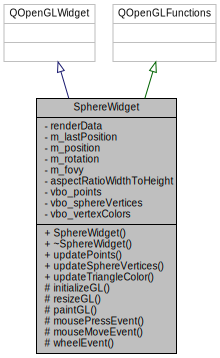
\includegraphics[width=292pt]{class_sphere_widget__inherit__graph}
\end{center}
\end{figure}


Collaboration diagram for Sphere\+Widget\+:
\nopagebreak
\begin{figure}[H]
\begin{center}
\leavevmode
\includegraphics[width=292pt]{class_sphere_widget__coll__graph}
\end{center}
\end{figure}
\subsection*{Public Member Functions}
\begin{DoxyCompactItemize}
\item 
\mbox{\Hypertarget{class_sphere_widget_a6ee7b3a4b58e5d62fb1c901aafdd1790}\label{class_sphere_widget_a6ee7b3a4b58e5d62fb1c901aafdd1790}} 
{\bfseries Sphere\+Widget} (Q\+Widget $\ast$parent=0)
\item 
\mbox{\Hypertarget{class_sphere_widget_a692ca1c1e7556f6abd7b5f6a49a2557c}\label{class_sphere_widget_a692ca1c1e7556f6abd7b5f6a49a2557c}} 
void {\bfseries update\+Points} ()
\item 
\mbox{\Hypertarget{class_sphere_widget_a7d132800fb4d6b7b925c253679bb6445}\label{class_sphere_widget_a7d132800fb4d6b7b925c253679bb6445}} 
void {\bfseries update\+Sphere\+Vertices} ()
\item 
\mbox{\Hypertarget{class_sphere_widget_a871c5252a7a218c5d405be5dfc3dbfa1}\label{class_sphere_widget_a871c5252a7a218c5d405be5dfc3dbfa1}} 
void {\bfseries update\+Triangle\+Color} ()
\end{DoxyCompactItemize}
\subsection*{Protected Member Functions}
\begin{DoxyCompactItemize}
\item 
\mbox{\Hypertarget{class_sphere_widget_a323d335cf261b7156da1a59aaf28c40c}\label{class_sphere_widget_a323d335cf261b7156da1a59aaf28c40c}} 
virtual void {\bfseries initialize\+GL} () override
\item 
\mbox{\Hypertarget{class_sphere_widget_aaf11c928f52c91d7f60317922df7ca73}\label{class_sphere_widget_aaf11c928f52c91d7f60317922df7ca73}} 
virtual void {\bfseries resize\+GL} (int w, int h) override
\item 
\mbox{\Hypertarget{class_sphere_widget_a122b798a2eb0c251f53671009abdf8c8}\label{class_sphere_widget_a122b798a2eb0c251f53671009abdf8c8}} 
virtual void {\bfseries paint\+GL} () override
\item 
\mbox{\Hypertarget{class_sphere_widget_ac658d6e1cdc99280ecff045f92fe1ba3}\label{class_sphere_widget_ac658d6e1cdc99280ecff045f92fe1ba3}} 
virtual void {\bfseries mouse\+Press\+Event} (Q\+Mouse\+Event $\ast$event) override
\item 
\mbox{\Hypertarget{class_sphere_widget_aef63eed14a55be78015576296dce516e}\label{class_sphere_widget_aef63eed14a55be78015576296dce516e}} 
virtual void {\bfseries mouse\+Move\+Event} (Q\+Mouse\+Event $\ast$event) override
\item 
\mbox{\Hypertarget{class_sphere_widget_aaecd84d746763a4bd6f46a6d55a36d84}\label{class_sphere_widget_aaecd84d746763a4bd6f46a6d55a36d84}} 
virtual void {\bfseries wheel\+Event} (Q\+Wheel\+Event $\ast$event) override
\end{DoxyCompactItemize}


\subsection{Detailed Description}
A custom Open\+G\+L\+Widget to render the scene from data collected inside the \hyperlink{class_render_data}{Render\+Data} singleton. 

The documentation for this class was generated from the following files\+:\begin{DoxyCompactItemize}
\item 
spherewidget.\+h\item 
spherewidget.\+cpp\end{DoxyCompactItemize}

\chapter{File Documentation}
\hypertarget{main_8cpp}{}\section{main.\+cpp File Reference}
\label{main_8cpp}\index{main.\+cpp@{main.\+cpp}}
{\ttfamily \#include \char`\"{}mainwindow.\+h\char`\"{}}\newline
{\ttfamily \#include $<$Q\+Application$>$}\newline
\subsection*{Functions}
\begin{DoxyCompactItemize}
\item 
int \hyperlink{main_8cpp_a0ddf1224851353fc92bfbff6f499fa97}{main} (int argc, char $\ast$argv\mbox{[}$\,$\mbox{]})
\end{DoxyCompactItemize}


\subsection{Function Documentation}
\mbox{\Hypertarget{main_8cpp_a0ddf1224851353fc92bfbff6f499fa97}\label{main_8cpp_a0ddf1224851353fc92bfbff6f499fa97}} 
\index{main.\+cpp@{main.\+cpp}!main@{main}}
\index{main@{main}!main.\+cpp@{main.\+cpp}}
\subsubsection{\texorpdfstring{main()}{main()}}
{\footnotesize\ttfamily int main (\begin{DoxyParamCaption}\item[{int}]{argc,  }\item[{char $\ast$}]{argv\mbox{[}$\,$\mbox{]} }\end{DoxyParamCaption})}


\hypertarget{mainwindow_8cpp}{}\section{mainwindow.\+cpp File Reference}
\label{mainwindow_8cpp}\index{mainwindow.\+cpp@{mainwindow.\+cpp}}
{\ttfamily \#include \char`\"{}mainwindow.\+h\char`\"{}}\newline
{\ttfamily \#include \char`\"{}ui\+\_\+mainwindow.\+h\char`\"{}}\newline
{\ttfamily \#include $<$Q\+File\+Dialog$>$}\newline
Include dependency graph for mainwindow.\+cpp\+:\nopagebreak
\begin{figure}[H]
\begin{center}
\leavevmode
\includegraphics[width=350pt]{d1/dd5/mainwindow_8cpp__incl}
\end{center}
\end{figure}

\hypertarget{mainwindow_8h}{}\section{mainwindow.\+h File Reference}
\label{mainwindow_8h}\index{mainwindow.\+h@{mainwindow.\+h}}
{\ttfamily \#include \char`\"{}resources/colormaps\+\_\+matplotlib.\+h\char`\"{}}\newline
{\ttfamily \#include $<$Q\+Main\+Window$>$}\newline
{\ttfamily \#include $<$Q\+Open\+G\+L\+Widget$>$}\newline
{\ttfamily \#include \char`\"{}spherewidget.\+h\char`\"{}}\newline
{\ttfamily \#include \char`\"{}renderdata.\+h\char`\"{}}\newline
Include dependency graph for mainwindow.\+h\+:
\nopagebreak
\begin{figure}[H]
\begin{center}
\leavevmode
\includegraphics[width=350pt]{mainwindow_8h__incl}
\end{center}
\end{figure}
This graph shows which files directly or indirectly include this file\+:
\nopagebreak
\begin{figure}[H]
\begin{center}
\leavevmode
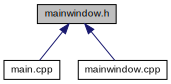
\includegraphics[width=244pt]{mainwindow_8h__dep__incl}
\end{center}
\end{figure}
\subsection*{Classes}
\begin{DoxyCompactItemize}
\item 
class \hyperlink{class_main_window}{Main\+Window}
\end{DoxyCompactItemize}
\subsection*{Namespaces}
\begin{DoxyCompactItemize}
\item 
 \hyperlink{namespace_ui}{Ui}
\end{DoxyCompactItemize}

\hypertarget{renderdata_8cpp}{}\section{renderdata.\+cpp File Reference}
\label{renderdata_8cpp}\index{renderdata.\+cpp@{renderdata.\+cpp}}
{\ttfamily \#include \char`\"{}renderdata.\+h\char`\"{}}\newline
Include dependency graph for renderdata.\+cpp\+:\nopagebreak
\begin{figure}[H]
\begin{center}
\leavevmode
\includegraphics[width=350pt]{df/da9/renderdata_8cpp__incl}
\end{center}
\end{figure}

\hypertarget{renderdata_8h}{}\section{renderdata.\+h File Reference}
\label{renderdata_8h}\index{renderdata.\+h@{renderdata.\+h}}
{\ttfamily \#include $<$list$>$}\newline
{\ttfamily \#include $<$vector$>$}\newline
{\ttfamily \#include $<$Q\+Vector3D$>$}\newline
{\ttfamily \#include $<$Q\+String$>$}\newline
{\ttfamily \#include $<$cnpy.\+h$>$}\newline
{\ttfamily \#include \char`\"{}icosphere.\+h\char`\"{}}\newline
{\ttfamily \#include \char`\"{}resources/colormaps\+\_\+matplotlib.\+h\char`\"{}}\newline
{\ttfamily \#include \char`\"{}spheredepthdata.\+h\char`\"{}}\newline
Include dependency graph for renderdata.\+h\+:
\nopagebreak
\begin{figure}[H]
\begin{center}
\leavevmode
\includegraphics[width=350pt]{renderdata_8h__incl}
\end{center}
\end{figure}
This graph shows which files directly or indirectly include this file\+:
\nopagebreak
\begin{figure}[H]
\begin{center}
\leavevmode
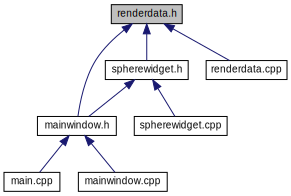
\includegraphics[width=350pt]{renderdata_8h__dep__incl}
\end{center}
\end{figure}
\subsection*{Classes}
\begin{DoxyCompactItemize}
\item 
class \hyperlink{class_render_data}{Render\+Data}
\end{DoxyCompactItemize}

\hypertarget{colormaps__matplotlib_8cpp}{}\section{resources/colormaps\+\_\+matplotlib.cpp File Reference}
\label{colormaps__matplotlib_8cpp}\index{resources/colormaps\+\_\+matplotlib.\+cpp@{resources/colormaps\+\_\+matplotlib.\+cpp}}
{\ttfamily \#include \char`\"{}resources/colormaps\+\_\+matplotlib.\+h\char`\"{}}\newline
Include dependency graph for colormaps\+\_\+matplotlib.\+cpp\+:\nopagebreak
\begin{figure}[H]
\begin{center}
\leavevmode
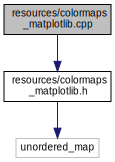
\includegraphics[width=187pt]{colormaps__matplotlib_8cpp__incl}
\end{center}
\end{figure}

\hypertarget{colormaps__matplotlib_8h}{}\section{resources/colormaps\+\_\+matplotlib.h File Reference}
\label{colormaps__matplotlib_8h}\index{resources/colormaps\+\_\+matplotlib.\+h@{resources/colormaps\+\_\+matplotlib.\+h}}
{\ttfamily \#include $<$unordered\+\_\+map$>$}\newline
Include dependency graph for colormaps\+\_\+matplotlib.\+h\+:
\nopagebreak
\begin{figure}[H]
\begin{center}
\leavevmode
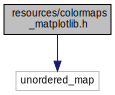
\includegraphics[width=187pt]{colormaps__matplotlib_8h__incl}
\end{center}
\end{figure}
This graph shows which files directly or indirectly include this file\+:
\nopagebreak
\begin{figure}[H]
\begin{center}
\leavevmode
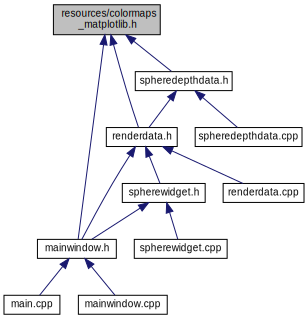
\includegraphics[width=350pt]{colormaps__matplotlib_8h__dep__incl}
\end{center}
\end{figure}
\subsection*{Namespaces}
\begin{DoxyCompactItemize}
\item 
 \hyperlink{namespacecm}{cm}
\end{DoxyCompactItemize}
\subsection*{Enumerations}
\begin{DoxyCompactItemize}
\item 
enum \hyperlink{namespacecm_aabaf84796e8a93bd6adca4c5bdea5311}{cm\+::\+Color\+Map\+Name} \{ \newline
\hyperlink{namespacecm_aabaf84796e8a93bd6adca4c5bdea5311a64c2ad47aeb457c258518a5318ed071d}{cm\+::\+Color\+Map\+Name\+::\+Cividis} = 0, 
\hyperlink{namespacecm_aabaf84796e8a93bd6adca4c5bdea5311a8bb279f735c1d9c831e935cca2613b58}{cm\+::\+Color\+Map\+Name\+::\+Inferno} = 1, 
\hyperlink{namespacecm_aabaf84796e8a93bd6adca4c5bdea5311a1b62e99f86d45e754e5e79d9fa9dfcde}{cm\+::\+Color\+Map\+Name\+::\+Magma} = 2, 
\hyperlink{namespacecm_aabaf84796e8a93bd6adca4c5bdea5311ab20a4217acaf4316739c6a5f6679ef60}{cm\+::\+Color\+Map\+Name\+::\+Plasma} = 3, 
\newline
\hyperlink{namespacecm_aabaf84796e8a93bd6adca4c5bdea5311a6f53bfe04e78da893ba0c4f35ba6847e}{cm\+::\+Color\+Map\+Name\+::\+Turbo} = 4, 
\hyperlink{namespacecm_aabaf84796e8a93bd6adca4c5bdea5311a951ee92ee5e947e1e7e1cb6376523c1a}{cm\+::\+Color\+Map\+Name\+::\+Viridis} = 5
 \}
\end{DoxyCompactItemize}
\subsection*{Variables}
\begin{DoxyCompactItemize}
\item 
const std\+::unordered\+\_\+map$<$ std\+::string, Color\+Map\+Name $>$ \hyperlink{namespacecm_a15083c75e20e3cb25b34ac29a4d66413}{cm\+::q\+String\+To\+Color\+Enum}
\item 
const float \hyperlink{namespacecm_a6c7ebc740c952f5ae2569bbc4d6b0ba3}{cm\+::\+\_\+magma\+\_\+data} \mbox{[}3 $\ast$256\mbox{]}
\item 
const float \hyperlink{namespacecm_abd85098a9455ec3b6a1367e717904d81}{cm\+::\+\_\+inferno\+\_\+data} \mbox{[}3 $\ast$256\mbox{]}
\item 
const float \hyperlink{namespacecm_a5e6bdf45c99146f14941db900036b42c}{cm\+::\+\_\+plasma\+\_\+data} \mbox{[}3 $\ast$256\mbox{]}
\item 
const float \hyperlink{namespacecm_af931122787ac6cf5d5c8d834adcb3fc8}{cm\+::\+\_\+viridis\+\_\+data} \mbox{[}3 $\ast$256\mbox{]}
\item 
const float \hyperlink{namespacecm_a9aebd281c6d694ef79eb8f989866ff6d}{cm\+::\+\_\+cividis\+\_\+data} \mbox{[}3 $\ast$256\mbox{]}
\item 
const float \hyperlink{namespacecm_a1394411b557deb7b6f8c58a9c39ff4a3}{cm\+::\+\_\+turbo\+\_\+data} \mbox{[}3 $\ast$256\mbox{]}
\end{DoxyCompactItemize}

\hypertarget{spheredepthdata_8cpp}{}\section{spheredepthdata.\+cpp File Reference}
\label{spheredepthdata_8cpp}\index{spheredepthdata.\+cpp@{spheredepthdata.\+cpp}}
{\ttfamily \#include \char`\"{}spheredepthdata.\+h\char`\"{}}\newline
Include dependency graph for spheredepthdata.\+cpp\+:\nopagebreak
\begin{figure}[H]
\begin{center}
\leavevmode
\includegraphics[width=350pt]{d0/d3f/spheredepthdata_8cpp__incl}
\end{center}
\end{figure}

\hypertarget{spheredepthdata_8h}{}\section{spheredepthdata.\+h File Reference}
\label{spheredepthdata_8h}\index{spheredepthdata.\+h@{spheredepthdata.\+h}}
{\ttfamily \#include $<$vector$>$}\newline
{\ttfamily \#include $<$algorithm$>$}\newline
{\ttfamily \#include $<$Q\+Vector3D$>$}\newline
{\ttfamily \#include \char`\"{}resources/colormaps\+\_\+matplotlib.\+h\char`\"{}}\newline
Include dependency graph for spheredepthdata.\+h\+:\nopagebreak
\begin{figure}[H]
\begin{center}
\leavevmode
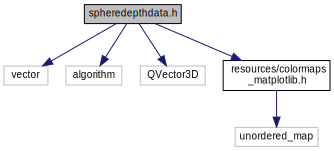
\includegraphics[width=350pt]{spheredepthdata_8h__incl}
\end{center}
\end{figure}
This graph shows which files directly or indirectly include this file\+:\nopagebreak
\begin{figure}[H]
\begin{center}
\leavevmode
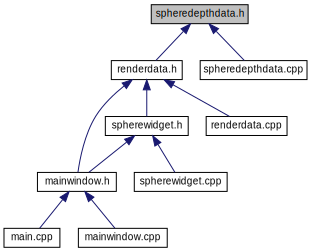
\includegraphics[width=350pt]{spheredepthdata_8h__dep__incl}
\end{center}
\end{figure}
\subsection*{Classes}
\begin{DoxyCompactItemize}
\item 
struct \hyperlink{struct_sphere_depth_data}{Sphere\+Depth\+Data}
\end{DoxyCompactItemize}

\hypertarget{spherewidget_8cpp}{}\section{spherewidget.\+cpp File Reference}
\label{spherewidget_8cpp}\index{spherewidget.\+cpp@{spherewidget.\+cpp}}
{\ttfamily \#include \char`\"{}spherewidget.\+h\char`\"{}}\newline
Include dependency graph for spherewidget.\+cpp\+:
\nopagebreak
\begin{figure}[H]
\begin{center}
\leavevmode
\includegraphics[width=350pt]{spherewidget_8cpp__incl}
\end{center}
\end{figure}

\hypertarget{spherewidget_8h}{}\section{spherewidget.\+h File Reference}
\label{spherewidget_8h}\index{spherewidget.\+h@{spherewidget.\+h}}
{\ttfamily \#include $<$Q\+Open\+G\+L\+Widget$>$}\newline
{\ttfamily \#include $<$Q\+Open\+G\+L\+Functions$>$}\newline
{\ttfamily \#include $<$Q\+Mouse\+Event$>$}\newline
{\ttfamily \#include $<$Q\+Open\+G\+L\+Buffer$>$}\newline
{\ttfamily \#include $<$vector$>$}\newline
{\ttfamily \#include $<$math.\+h$>$}\newline
{\ttfamily \#include $<$G\+L/glu.\+h$>$}\newline
{\ttfamily \#include \char`\"{}renderdata.\+h\char`\"{}}\newline
{\ttfamily \#include $<$iostream$>$}\newline
Include dependency graph for spherewidget.\+h\+:\nopagebreak
\begin{figure}[H]
\begin{center}
\leavevmode
\includegraphics[width=350pt]{spherewidget_8h__incl}
\end{center}
\end{figure}
This graph shows which files directly or indirectly include this file\+:\nopagebreak
\begin{figure}[H]
\begin{center}
\leavevmode
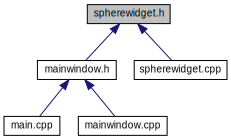
\includegraphics[width=304pt]{spherewidget_8h__dep__incl}
\end{center}
\end{figure}
\subsection*{Classes}
\begin{DoxyCompactItemize}
\item 
class \hyperlink{class_sphere_widget}{Sphere\+Widget}
\end{DoxyCompactItemize}
\subsection*{Macros}
\begin{DoxyCompactItemize}
\item 
\#define \hyperlink{spherewidget_8h_a525335710b53cb064ca56b936120431e}{\+\_\+\+U\+S\+E\+\_\+\+M\+A\+T\+H\+\_\+\+D\+E\+F\+I\+N\+ES}
\end{DoxyCompactItemize}


\subsection{Macro Definition Documentation}
\mbox{\Hypertarget{spherewidget_8h_a525335710b53cb064ca56b936120431e}\label{spherewidget_8h_a525335710b53cb064ca56b936120431e}} 
\index{spherewidget.\+h@{spherewidget.\+h}!\+\_\+\+U\+S\+E\+\_\+\+M\+A\+T\+H\+\_\+\+D\+E\+F\+I\+N\+ES@{\+\_\+\+U\+S\+E\+\_\+\+M\+A\+T\+H\+\_\+\+D\+E\+F\+I\+N\+ES}}
\index{\+\_\+\+U\+S\+E\+\_\+\+M\+A\+T\+H\+\_\+\+D\+E\+F\+I\+N\+ES@{\+\_\+\+U\+S\+E\+\_\+\+M\+A\+T\+H\+\_\+\+D\+E\+F\+I\+N\+ES}!spherewidget.\+h@{spherewidget.\+h}}
\subsubsection{\texorpdfstring{\+\_\+\+U\+S\+E\+\_\+\+M\+A\+T\+H\+\_\+\+D\+E\+F\+I\+N\+ES}{\_USE\_MATH\_DEFINES}}
{\footnotesize\ttfamily \#define \+\_\+\+U\+S\+E\+\_\+\+M\+A\+T\+H\+\_\+\+D\+E\+F\+I\+N\+ES}



Definition at line 12 of file spherewidget.\+h.


%--- End generated contents ---

% Index
\backmatter
\newpage
\phantomsection
\clearemptydoublepage
\addcontentsline{toc}{chapter}{Index}
\printindex

\end{document}
